
\Tlabel{CP1}\TChapter{Marco teórico}{gama}
\ \\\\
%---------------------------------Introducción--------------------------------%
En este capítulo se expondrán de manera detallada y ordenada el conjunto de conocimientos que permitirán comprender y analizar el tema propuesto. \\

La Figura \ref{fig:MarcoT} muestra los campos abarcados por la investigación.
A continuación cada área sera desarrollada con los conceptos de interés para la solución propuesta.

\begin{figure}[H]
	\centering
	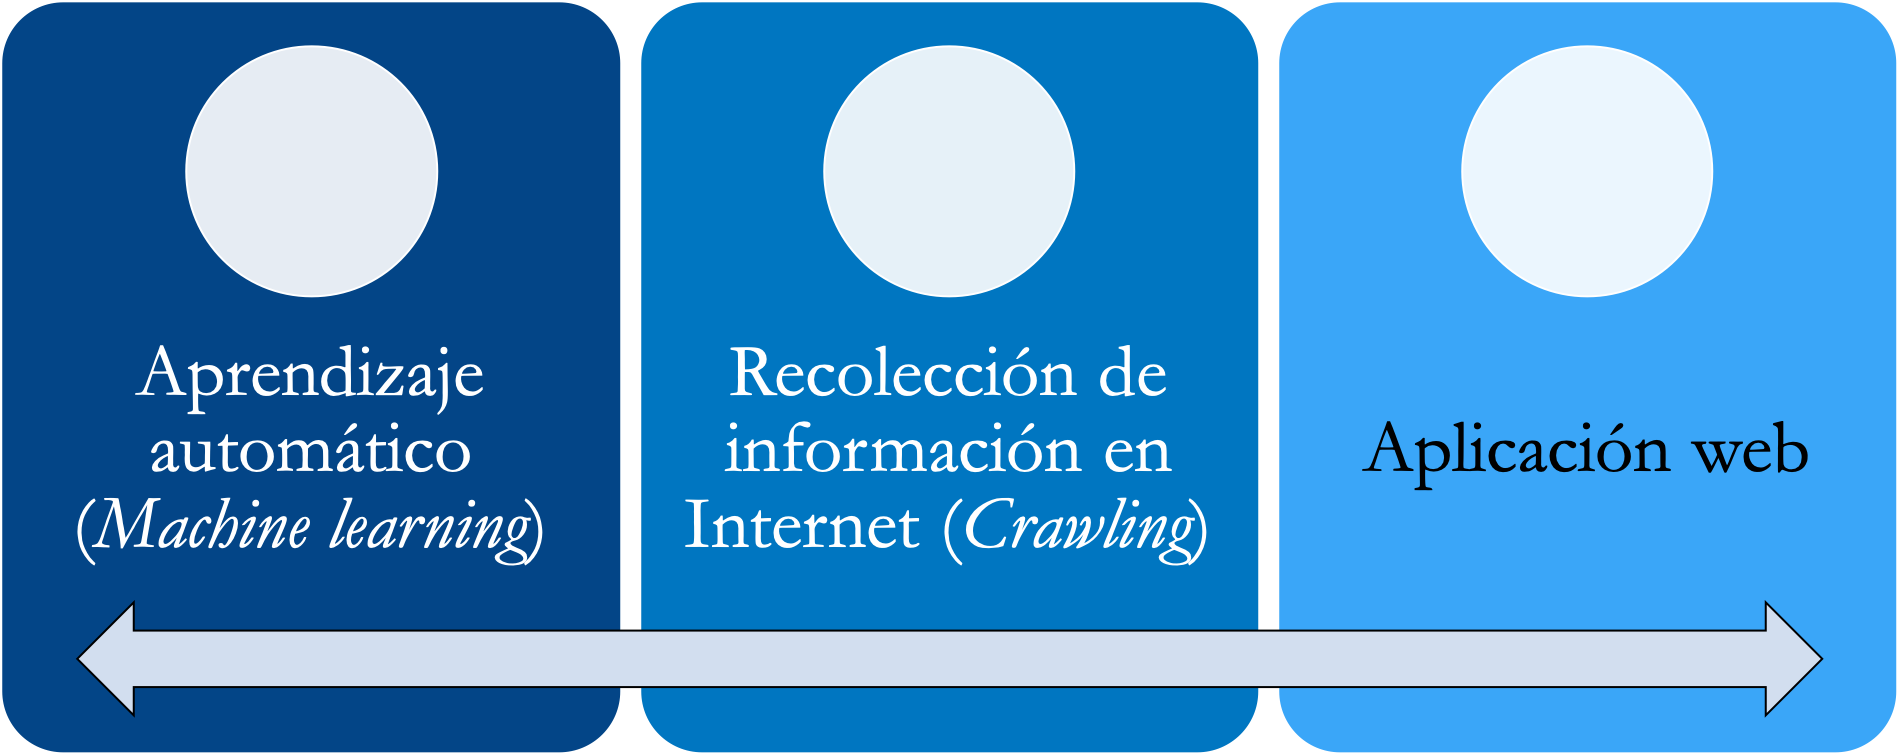
\includegraphics[scale=.35]{imagenes/Capitulo3/Marco.png}
	\caption{Campo de estudio}
	\label{fig:MarcoT}
\end{figure}

%---------------------------------Conceptos-------------------------------------%

%----------------------------------------Aprendizaje automático-------------------------------%
%---------------------------------------------------------------------------------------------%

\MTtitle{Aprendizaje automático}


%------------------------------------Inteligencia Artificial-------------------------------%
\section{Inteligencia Artificial}

Son muchas las definiciones que se encuentran de la inteligencia artificial o IA, en sus inicios se propone como las  actividades asociadas al pensamiento humano, tareas como, toma de decisiones, resolución de problemas y aprendizaje \citep{CT19}. Con el paso de los años se ha acuñado una definición mas completa: ``la Inteligencia Artificial es una ciencia orientada al diseño y construcción de máquinas que implementen tareas propias de humanos dotados de inteligencia'' \citep{CT1}.\\


Esta ciencia contribuye en el desarrollo de diversos campos de investigación como, Redes neuronales, Computación evolutiva, Algoritmos genéticos, Programación Genética, Teoría del caos. Además tiene un campo amplio de aplicaciones en la sociedad \citep{CT20}, a continuación se muestran algunos ejemplos:

\begin{itemize}
	\item \textbf{Vehículos robóticos}: Un auto robótico sin conductor llamado STANLEY aceleró a través del terreno de Mojave a 22 mph, terminando el curso de 132 millas primero para ganar el Gran Desafío DARPA 2005.

	\item \textbf{Reconocimiento de voz}: Un viajero que llama a \textit{United Airlines} para reservar un vuelo puede tener la conversación completa guiada por un sistema automático de reconocimiento de voz y gestión de diálogos.

	\item \textbf{Planificación y programación autónoma}: A cien millones de millas de la Tierra, el programa \textit{Remote Agent} de la NASA se convirtió en el primer programa autónomo de planificación a bordo para controlar la programación de operaciones de una nave espacial.

	\item \textbf{Robótica}: \textit{iRobot Corporation} ha vendido más de dos millones de aspiradoras robóticas \textit{Roomba} para uso doméstico.

	\item \textbf{Máquina traductora}: Un programa de computadora  traduce automáticamente del árabe al inglés.

\end{itemize} 

%------------------------------------Apredizje automático-------------------------------%
\section{Aprendizaje Automático}

EL Aprendizaje Automático es una rama de la Inteligencia Artificial; permite desarrollar algoritmos que tienen la capacidad de extrapolar (\textit{i.e} predecir) los cambios que se acontecen en una tarea específica \citep{CT2}.\\

EL campo utiliza una variedad de algoritmos que aprenden iterativamente de un conjunto de
datos para describir y predecir resultados. A medida en la cual los algoritmos de 
entrenamiento obtienen datos es posible obtener modelos más precisos. Existen cuatro clasificaciones en los métodos \citep{CT21}:

\begin{itemize}

	\item \textbf{Aprendizaje supervisado}: Se proporciona un conjunto de datos de entrenamiento con las respuestas correctas y, con base a este conjunto de 
	entrenamiento, el algoritmo se generaliza para responder correctamente a todas 
	las entradas posibles.

	\item \textbf{Aprendizaje no supervisado}: No se proporcionan datos de entrenamiento, el algoritmo intenta identificar similitudes entre las entradas para clasificar en conjuntos. El enfoque estadístico del aprendizaje no 
	supervisado se conoce como estimación de densidad.

	\item \textbf{Aprendizaje reforzado}: Está en algún lugar entre el aprendizaje supervisado y no supervisado. Se indica al algoritmo cuando la respuesta es incorrecta, sin embargo no se informa
	cómo corregirlo. Tiene que explorar y probar diferentes posibilidades hasta que resuelva 
	cómo obtener la respuesta correcta.

	\item \textbf{Aprendizaje evolutivo}: La evolución biológica puede verse como un proceso de aprendizaje: los organismos biológicos se adaptan para mejorar sus tasas de supervivencia 
	y la posibilidad de tener descendientes en su entorno. Este comportamiento es modelado, 
	usando un modelo física, el cual corresponde a una puntuación en la 
	solución actual.

\end{itemize}

Cabe mencionar que el método implementado en este trabajo es el aprendizaje supervisado, mas a delante se da una explicación detalla.\\

El aprendizaje automático se puede aplicar a una amplia gama de problemas comerciales, desde la detección de fraudes hasta la orientación al cliente y la recomendación de productos, al monitoreo industrial en tiempo real, el análisis de sentimientos y el diagnóstico médico. Puede asumir problemas que no pueden administrarse manualmente debido a la gran cantidad de datos que deben procesarse \citep{CT22}. Cuando se aplica a grandes conjuntos de datos, a veces puede encontrar relaciones tan sutiles que ninguna cantidad de escrutinio manual las descubriría nunca. Y cuando muchas de estas relaciones ``débiles'' se combinan, se convierten en predictores fuertes.


%------------------------------------Apredizje automático para texto------------------------%

\section[AI para texto]{Aprendizaje automático para texto}

La extracción de información útil con varios tipos de algoritmos estadísticos es denominado \textbf{Extracción de datos}( \textit{Text mining} ), \textbf{Analítica de texto} (\textit{Text analytics}) o \textbf{Aprendizaje automático para texto} (\textit{Machine learning for text}) \citep{CD1}. En los últimos años este campo ha incrementado por el desarrollo de la web, redes sociales, correos electrónicos, bibliotecas virtuales. Algunos ejemplos para obtener información son:


\begin{itemize}

	\item \textbf{Bibliotecas digitales}: El uso de la información electrónica ha superado la producción de libros y publicaciones impresas, este fenómeno ha proliferado la producción de bibliotecas digitales, estas pueden ser almacenadas y ser usadas para extraer información útil.

	\item \textbf{Noticias electrónicas}: Existe un movimiento masivo para pasar las noticias impresas hacía la publicación electrónica, esto permite que sean almacenadas para su análisis y extracción de información sobre eventos y perspectivas importantes. Sitios como \textit{Google news} etiquen las noticias para hacer recomendaciones al lector basado en su anterior comportamiento o intereses específicos.

	\item \textbf{\textit{Web and Web-enabled applications}}: La web contiene una gran cantidad de información en hipertexto, con links y otro tipo de recursos, la cual puede ser utilizada par el proceso de descubrimiento de nuevo conocimiento, al igual las \textit{Web-enabled applications}\footnote{\textbf{\textit{Web and Web-enabled applications}}: Aplicaciones de escritorio que son  accedidas remotamente des de un buscador como Internet explorer.} permiten obtener información que puede ser analizada.

	\item \textbf{Redes sociales}: Las redes sociales son un campo que está proliferando, debido a su naturaleza donde cada usuario contribuye con sus propias publicaciones.

\end{itemize}


Algunas de las aplicaciones son las siguientes:

\begin{itemize}

	\item Etiquetar la web, permite al usuario encontrar paginas de interés

	\item Los proveedores de correos, utilizan la información almacenada para mostrar publicidad de interés al usuario

	\item Algunas páginas ordenan su contenido de acuerdo a su importancia

	\item El análisis de las opiniones es un campo de importancia así como el análisis de sentimientos		

\end{itemize}



El orden de las palabras en un texto brindan un significado semántica el cual no puede ser inferido  solo con la frecuencia de las palabras. Sin embargo, se pueden hacer varias predicciones sin contemplar la semántica. Existen 2 tipos de representaciones que son populares en las aplicaciones de \textbf{text mining}:

\begin{itemize}
	
	\item \textbf{\textit{Text as a bag-of-words}}: Es la representación mas común. No se contempla el orden de las palabras el proceso. El conjunto de palabras en el documento se convierten en \textit{Sparse multidimentional reprentation}, el cual corresponde a la dimensión en esta representación. Se utiliza para la clasificación, sistemas de recomendación.

	\item \textbf{\textit{Text as a set of sequences}}: En esta representación se extraen sentencias, el orden de las palabras si importa. La unidad son sentencia o párrafos. Es utilizado en aplicaciones que necesitan un fuerte uzo de la semántica, esta área se acerca mucho al modelado de lenguaje y procesamiento del lenguaje natural

\end{itemize}

%------------------------------------Pre-procesamiento------------------------%

\section[Pre-procesamiento]{Pre-procesamiento}

El Pre-procesamiento es necesario para convertir el formato no estructurado en un formato estructurado \citep{CD1}.
A menudo el texto contiene información extraña como etiquetas, \textit{anchor text}\footnote{Es el texto mostrado en los enlaces o hipervínculos, \textbf{Texto de anclaje} en español.}, y otras características. En muchos casos las palabras son variaciones de otras (Sinónimos) por el tipo de redacción, el contexto, para eliminar redundancia. Algunas palabras simplemente tienen faltas de ortografía. El proceso de convertir una secuencia de caracteres en una secuencia de palabras(Tokens), es llamado \textbf{Tokenización}. Además por cada palabra repetida se crea un token, es decir al repetirse una palabra 3 veces, se crearán 3 tokens correspondientes. Alguno de los pasos mas comunes para el procesamiento de texto en bruto son los siguientes: 

\begin{itemize}

	\item \textbf{Extracción de texto}: En caso de recuperar información de la web, se tiene que limpiar el texto ya que contiene \textit{anchor text}, etiquetas.Se debe buscar los bloques que brinden información útil para el análisis, ya que algunos bloques contienen publicidad o información no relacionada. Para esto se tiene que realizar un \textbf{parseo}\footnote{Es la acción de analizar el texto de forma especializada} o técnicas de extracción especializadas.

	\item \textbf{Remover stop-words}: \textbf{Stop words}, son pronombres, \textit{articles} y preposiciones que deben ser removidas para mejorar la compresión del texto.

	\item  \textbf{Stemming, case-folding, punctuation}: Las palabras que derivan de la misma raíz como hundimiento, se hundió, se reducen a hundir. Una palabra puede tener diferentes significados dependiendo el contexto como la palabra \'Rosa\' puede hacer referencia a una flor o el nombre de una persona, por lo tanto se requiero la euristica del lenguaje específico para poder tomar una decisión en como debe ser interpretada. Los signos de puntuación como el guión medio deben ser tratados con mucho cuidado para realizar una buena tokenización.

	\item \textbf{\textit{Frequency-based normalization}}: Palabras con poca frecuencia son mas discriminatorias que las de alta frecuencia. Por lo tanto se pondera la importancia de los documentos con base al calculo de la \textbf{frecuencia inversa del documento}(\textit{fid}) en la colección. Si $\psi_i$ es el número de documentos en el cual la palabra aparece, y $\psi$ es el número total de documentos, la \textit{fid} se calcula como $log(\frac{\psi}{\psi_i})$. La importancia de un documento se calcula multiplicando la \textbf{frecuencia de término} (\textit{ft}) en el documento por la \textit{fid}. Mientras la \textit{ft} brinda la cantidad de veces  que una palabra aparece en el documento la \textit{fid} especifica la importancia en la colección; Se define como \textbf{ft-fid} o \textit{tf-idf} (Por su sigla en ingles \textit{Term frequency – Inverse document frequency}).

\end{itemize}


\subsection{Aprendizaje supervisado}

Los algoritmos de aprendizaje supervisado dependen de datos previamente etiquetados, es decir necesita de un entrenamiento para 
que el algoritmo pueda comprender los datos y con ello determinar que etiqueta debe asignarse a los nuevos datos 
en función del patron y asociando los patrones a los nuevos datos sin etiquetar. Después de ello, la maquina recibe 
un nuevo conjunto de datos para que el algoritmo de aprendizaje supervisado analice los datos y produzca un resultado 
correcto de los datos etiquetados \citep{CT4}.


%https://cleverdata.io/conceptos-basicos-machine-learning/

\subsubsection{Regresión logística}
La regresión logística es una técnica estadística multivariante que nos permite estimar la relación existente entre una variable dependiente 
no métrica (donde la variable es binaria o también conocida como dicotómica, es decir, solo va a dar como resultado dos alternativas posibles) 
y un conjunto de variables intependientes métricas o no métricas \citep{CT6}. Es útil para modelar la probabilidad de un evento ocurriendo como 
función de otros factores. El análisis de regresión logística se enmarca en el conjunto de Modelos Lineales Generalizados que usa como función de 
enlace la función logit. Las probabilidades que describen el posible resultado de un único ensayo se modelan, como una función de variables explicativas, 
utilizando una función logística.

La regresión logística es usada extensamente en las ciencias médicas y sociales. Otros nombres para regresión logística usados en varias áreas de 
aplicación incluyen modelo logístico, modelo logit, y clasificador de máxima entropía.


\subsubsection{Na{\"i}ve bayes}
Na{\"i}ve Bayes es un conjunto de algoritmos de aprendizaje supervisado que se basan en la aplicación del teorema de Bayes con "Na{\"i}ve" 
(Ingenuo) la cual es la supuesta de independencia condicional entre cada par de características dado el valor de la variable de clase. 

La clasificación Naive Bayes son aproximaciones probabilísticas, las cuales hacen especulaciones sobre como deben de ser 
generados los datos. Generalmente utilizan aprendizaje supervisado sobre el conjunto de entrenamiento para poder esimar los parámetros 
del modelo generativo, en tanto el conjunto de datos de entrada nuevos se realiza el teorema de Bayes, seleccionando la probable categoría 
que se ha generado \cite{CT7}.
\\
Todas las características extraídas que utilizan este clasificador son independientes entre sí. La ventaja de usar este clasificador es que 
funciona bien tanto con datos numéricos como con datos textuales y, además, es más fácil de implementar. La desventaja de este clasificador es 
que su rendimiento empeora cuando las características extraídas se correlacionan entre sí.

\subsubsection{Maquina de soporte vectorial}
Las maquinas de soporte vectorial son un conjunto de algoritmos de aprendizaje los cuales se basan en el uso de un espacio de funciones lineales, 
el cual se encuentra con mas dimensiones inducido por un kernel, en el que las hipotesis son las entradas para el algoritmo. \\
El algoritmo induce separadores lineales ya sea en el espacio original de los ejemplos de entrada, si los datos no son separabales se busca un hiperplano 
en el que si lo sean, se hace de forna implicita con las funciones kernel.\\

Estos métodos están propiamente relacionados con problemas de clasificación y regresión. Dado un conjunto de ejemplos de entrenamiento (de muestras) 
podemos etiquetar las clases y entrenar una SVM para construir un modelo que prediga la clase de una nueva muestra. Intuitivamente, una SVM es un modelo 
que representa a los puntos de muestra en el espacio, separando las clases a 2 espacios lo más amplios posibles mediante un hiperplano de separación definido 
como el vector entre los 2 puntos, de las 2 clases, más cercanos al que se llama vector soporte. Cuando las nuevas muestras se ponen en correspondencia con dicho 
modelo, en función de los espacios a los que pertenezcan, pueden ser clasificadas a una o la otra clase \citep{CT8}.

\subsubsection{Random forest}
Random forest es una combinación de árboles predictiroes, de modo que cada árbol depende de los valores de un vector 
aleatorio muestreado independientemente y con la misma distribución para cada uno de estos. Es una modificación sustancial de bagging que construye una 
larga colección de árboles no correlacionados y posteriormente los promedia \citep{CT9}.

\subsection{Aprendizaje no supervisado}
Los algoritmos de aprendizaje no supervisado no dependen de datos previamente etiquetados, por lo cual los algoritmos 
tienen la tarea de agrupar la información no clasificada según sus similitudes, patrones y diferencias sin ningún entrenamiento 
previó de datos, por lo cual aprenden gracias a la cantidad de datos que le son ingresadas con características propias de un 
objeto y con ello pueda determinar los resultados basados en los datos de entrada \citep{CT10}.
%https://towardsdatascience.com/supervised-machine-learning-classification-5e685fe18a6d

\section{Procesamiento de lenguaje natural}
El procesamiento de lenguaje natural es una disciplina de la Inteligencia Artificial que se ocupa de la formulación e 
investigación de mecanismos computacionales para la comunicación entre personas y maquinas mediante el uso de Lenguajes 
Naturales.

El procesamiento del lenguaje natural incluye diferentes técnicas para interpretar el lenguaje humano, que van desde los métodos 
estadísticos y del aprendizaje basado en máquina hasta los enfoques basados en reglas y algorítmicos. Necesitamos una amplia variedad 
de métodos porque los datos basados en texto y en voz varían ampliamente, al igual que las aplicaciones prácticas. 

Las tareas básicas de NLP incluyen la simbolización y el análisis sintáctico , lematización/derivación, etiquetado de la parte del 
habla, detección del lenguaje e identificación de relaciones semánticas. Si alguna vez creó diagramas de enunciados en la primaria, 
ya ha realizado estas tareas de forma manual antes. 

En términos generales, las tareas NLP dividen el lenguaje en piezas elementales más cortas, intentan entender las relaciones entre 
las piezas y exploran cómo funcionan las piezas juntas para crear significado \citep{CT11}.

Estas tareas implícitas se utilizan a menudo en recursos NLP de más alto nivel, como:
\begin{itemize}
	\item Categorización de contenido. Un resumen del documento basado en la lingüística, 
	incluyendo búsqueda e indización, alertas de contenido y detección de duplicación.
	\item Descubrimiento y modelado de temas. Capture con precisión el significado y temas en colecciones de texto, y 
	aplique analítica avanzada a texto, como optimización y pronósticos.
	\item Extracción contextual. Extraiga automáticamente información estructurada de fuentes basadas en texto.
	\item Análisis de sentimiento. Identificación del estado de ánimo u opiniones subjetivas en grandes cantidades de 
	texto, incluyendo minería de sentimiento y opiniones promedio. 
	\item Conversión de habla a texto y de texto a habla. Transformación de comandos de voz en texto escrito y viceversa. 
	\item Sumarización de documentos. Generación automática de sinopsis de grandes cuerpos de texto.
	\item Traducción basada en máquina. Traducción automática de texto o habla de un idioma a otro.
\end{itemize}

%\subsection{Lenguaje}
%El lenguaje es un medio de comunicación a traves de de un sistema de símbolos \cite{dieciseis}.
%La Real Academía Española define al lenguaje como la facultad del ser humano de expresarse y comunicarse con los demás 
%a través del sonido articulado o de otros sistemas de signos.

\subsection{Tokenización}
Es el proceso que descompone los textos de una colección en sus unidades mínimas, las palabras
o términos propiamente dichos. A tales elementos se les denomina tokens que conforman una lista de
ítems que se utiliza para su análisis estadístico, ling{\"u}ístico, de almacenamiento y posteriormente de
recuperación de información. Los tokens a su vez pueden ser identificados mediante una codificación
ASCII o en su defecto hexadecimal, con el objeto de facilitar la identificación uno a uno cada caracter
que compone la palabra. De hecho, este proceso permite la identificación de cadenas de caracteres de
forma unívoca, de cara a posteriores tratamientos de depuración, eliminación de signos de puntiación
o la reducción morfológica \citep{CT12}.

Ejemplo  (\ref{tabla:sencilla}): Hoy es un gran día para salir.

\begin{table}[htbp]
	\begin{center}
	\begin{tabular}{|lrrccccc|}
		\hline
		ID & 1 & 2 & 3 & 4 & 5 & 6 & 7 \\ 
		Token & Hoy & es & un & gran & día & para & salir \\ \hline
		\hline
	\end{tabular}
	\caption{Ejemplo de tokenización}
	\label{tabla:sencilla}
	\end{center}
	
\end{table}


\subsection{Lematización}
Es el proceso lingüstico que, dada una palabra flexionada se encuentra su
lema. Una palabra flexionada es cuando esta en el plural, en femenino conjugada,
diminutivo o en superlativo. El lema es la palabra que esta en singular para
sustantivo, singular masculino para adjetivo e infinitivo para un verbo \citep{CT13}. Ejemplo:

	\begin{itemize}
		\item amigos, amiga, amiguitos-> Amigo
		\item soy, son, es->Ser
	\end{itemize}

Cabe mencionar que existen diversos grados de lematización

	\begin{itemize}
		\item Mórfólogica: Es la anterior mente explicada
		\item Sintáctica: Toma encuenta el contexto donde se encuentra la palabra

	\end{itemize}

Una opción para lematizar es Freeling \citep{CT18}, este es un lematizador hecho por la
universidad de catalunia.

\section[Representación del t.]{Representación del texto}
Los métodos de Aprendizaje Automático requieren que la información de la cual aprenderán esté representada en un
formato que facilite su procesamiento. Generalmente esta representación es mediante vectores de valores numéricos. 
Cuando se requiere utilizar estos métodos con información en forma de texto, dicha
información debe ser transformada para generar una representación más adecuada. 

\section{Corpus}
Se le llama corpus a la recopilación de un conjunto de textos, de materiales escritos y/o hablados, 
agrupados bajo un conjunto de criterios mínimos, para realizar ciertos análisis lingüísticos.

%-------------------Recolección de información de Internet------------------------------------%
%---------------------------------------------------------------------------------------------%
\MTtitle{Recolección de información de Internet}

\section{Crawler}
Un crawler \citep{CT14} es una herramienta la cual analiza sitios web, permitiendo recolectar 
las páginas web para así posteriormente extraer la información que contengan. Un crawler también 
conocido como como robot o spider, es un sistema para la descarga masiva de páginas web. Son uno de 
los componentes principales de los motores de búsqueda web, los sistemas que reúnen un conjunto de 
páginas web, las indexan y permiten a los usuarios realizar consultas contra el índice y encontrar las 
páginas web que coincidan con las consultas.



%------------------------------------Aplicación web-------------------------------------------%
%---------------------------------------------------------------------------------------------%
\MTtitle{Aplicación web}


\section{Sitios web}
Un sitio web \citep{CT15} es un conjunto de páginas web interconectadas y de acceso público que comparten 
un solo nombre de dominio. Los sitios web pueden ser creados y mantenidos por un individuo, grupo, empresa 
u organización para cumplir una variedad de propósitos. Todos estos sitios constituyen la World Wide Web. 

\subsection{Página web}
Una página web es un documento electrónico el cual forma parte de la WWW (\textit{World Wide Web}) generalmente 
construido en el lenguaje HTML (\textit{Hyper Text Markup Language}). Este documento puede contener enlaces que nos 
direcciona a otra página web. Para visualizar una página web es necesario de un browser o un navegador \citep{CT16}. 
Dentro de las páginas web podemos encontrar un sinfin de sitios los cuales pueden ser de nuestro interés.

\subsection{Blog}
Un blog es una página web en la cual el usuario no necesita conocimientos específicos del medio electrónico ni del 
formato digital para poder aportar contenidos de forma inmediata, ágil y constante desde cualquier punto de conexión 
a Internet \citep{CT17}. En un blog el usuario puede compartir cualquier tipo de información que sea de su agrado, 
teniendo una mayor libertad de expresión lo cual permite que otras personas compartan y comenten su manera de expresarse.

\subsection{Foro}
Un foro es una herramienta de comunicación asíncrona. Los foros permiten la comunicación de los participantes desde 
cualquier lugar en el que  esté  disponible  una  conexión  a Internet  sin  que  éstos  tengan  que  estar dentro del 
sistema al mismo tiempo, de ahí su naturaleza asíncrona. Brindando una mayor interacción entre distintos 
participantes y permitiendo conocer la opinión sobre un tema de distintas personas.


